\documentclass[../document.tex]{subfiles}
\begin{document}
\section{Interpretability}
In this section, we will evaluate the model's prediction to better understand it. We will find if there are any features in the patches that can confuse it and if the model's output is robust.
First, we will introduce on technique used to highlight the region of the input image that contribute the most to the model predictions. Then, we will use it on the data from the \emph{Quarry} test set to find out the patches were the model fails and analyze them.

Later, we will work with custom created patches with different features, walls, bumps, etc, to test the robustness of the model by comparing its predictions to the real data gathered from the simulator.

\subsubsection{Grad-CAM}
Informally, Grad-CAM \cite{gradcam} to produce "visual explanations" for convolutional neural networks. It uses the gradient flowing into the last convolution layer to highlight a region of interested in the image that contribute the most to the final prediction. 

\begin{figure}[H]
    \centering
    \begin{subfigure}[b]{1\textwidth}
        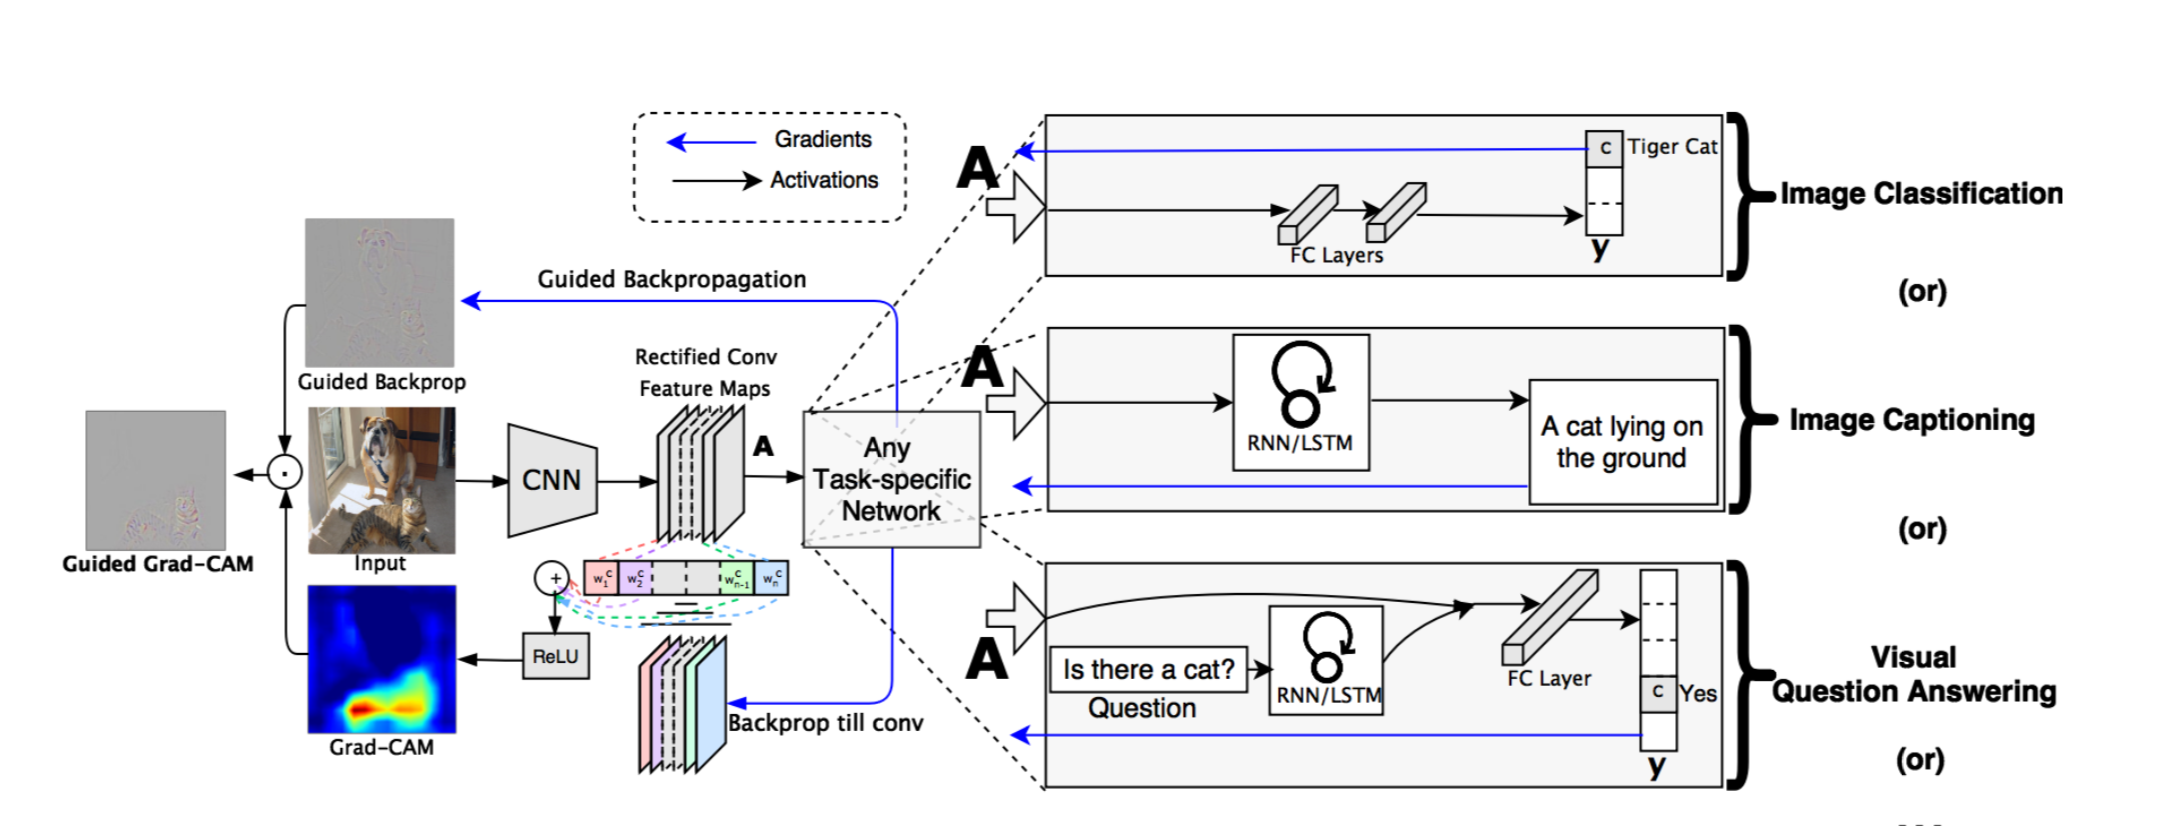
\includegraphics[width=\linewidth]{../img/5/grad_cam1.png}
    \end{subfigure}
\caption{Grad-CAM procedure on an input image \cite{gradcam}.}
\end{figure}

In detail, the output with respect to a target class is backpropagate while storing the gradient and the output at a given layer, in our case the last convolution. Then it is performed a global average of the saved gradient keeping the channel dimension in order to get a 1-d tensor, this will represent the importance of each channel in the target convolutional layer. We  each element of the convolutional layer outputs is multiplyed with the averaged gradients to create the grad cam. This whole procedure is fast and it is architecture independent, meaning we can use it on any type of CNN.



\end{document}z